\documentclass{standalone}
\usepackage{tikz,xcolor,amsmath}
\begin{document}
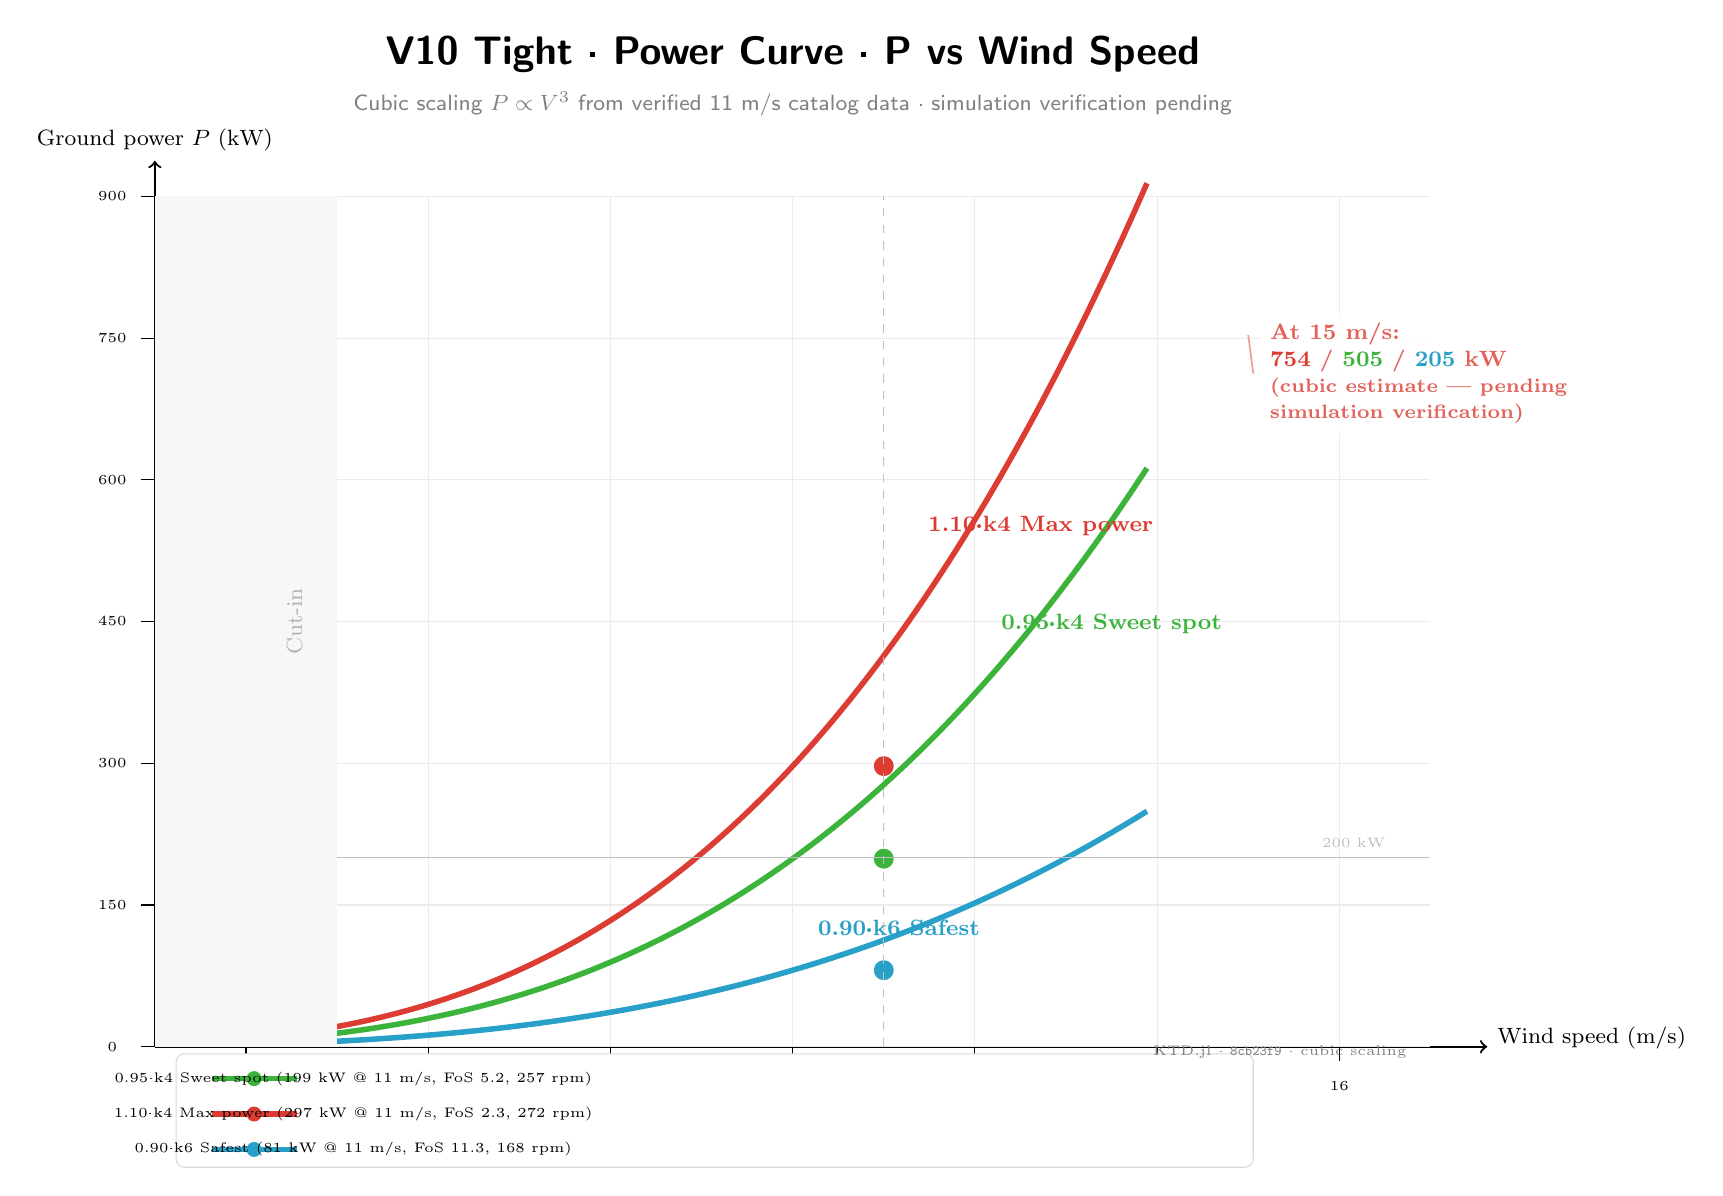
\begin{tikzpicture}[scale=0.90]

% ── Title ──
\node[font=\Large\sffamily\bfseries] at (11.0, 16.0) {V10 Tight · Power Curve · P vs Wind Speed};
\node[font=\footnotesize\sffamily, black!50] at (11.0, 15.3) {Cubic scaling $P \propto V^3$ from verified 11 m/s catalog data · simulation verification pending};

% ── Axes: x=2.0+(V-3)*18/14, y=2.0+P*12/900 ──
\draw[->, thick] (2.0, 2.0) -- (20.8, 2.0) node[right, font=\footnotesize, yshift=3pt] {Wind speed (m/s)};
\draw[->, thick] (2.0, 2.0) -- (2.0, 14.5) node[above, font=\footnotesize] {Ground power $P$ (kW)};

% Grid
\foreach \v in {4,6,8,10,12,14,16} {
  \pgfmathsetmacro{\x}{2.0 + (\v-3.0)*18/14}
  \draw[black!8] (\x, 2.0) -- (\x, 14.0);
  \draw (\x, 1.8) -- (\x, 2.0);
  \node[font=\tiny] at (\x, 1.45) {\v};
}
\foreach \p in {0,150,300,450,600,750,900} {
  \pgfmathsetmacro{\y}{2.0 + \p*12/900}
  \draw[black!8] (2.0, \y) -- (20.0, \y);
  \draw (1.8, \y) -- (2.0, \y);
  \node[font=\tiny] at (1.4, \y) {\p};
}

% ── Helpers ──
\definecolor{sweet}{RGB}{60,180,60}
\definecolor{maxp}{RGB}{220,60,50}
\definecolor{safe}{RGB}{40,160,200}

% Sweet spot: P(V) = 199*(V/11)^3
\draw[sweet, line width=2pt, domain=3.5:16.0, samples=60, smooth] 
  plot (\x, {2.0 + 199*(\x/11.0)^3 * 12/900});
\node[sweet, font=\footnotesize\bfseries] at (15.5, {2.0 + 199*(14.0/11.0)^3*12/900 + 0.5}) {0.95·k4 Sweet spot};

% Max power: P(V) = 297*(V/11)^3
\draw[maxp, line width=2pt, domain=3.5:16.0, samples=60, smooth] 
  plot (\x, {2.0 + 297*(\x/11.0)^3 * 12/900});
\node[maxp, font=\footnotesize\bfseries] at (14.5, {2.0 + 297*(13.2/11.0)^3*12/900 + 0.5}) {1.10·k4 Max power};

% Safest: P(V) = 81*(V/11)^3
\draw[safe, line width=2pt, domain=3.5:16.0, samples=60, smooth] 
  plot (\x, {2.0 + 81*(\x/11.0)^3 * 12/900});
\node[safe, font=\footnotesize\bfseries] at (12.5, {2.0 + 81*(11.0/11.0)^3*12/900 + 0.6}) {0.90·k6 Safest};

% ═══════════════════════════════════════
% ANCHOR POINTS at 11 m/s (verified)
% ═══════════════════════════════════════
\pgfmathsetmacro{\vx}{2.0 + (11.0-3.0)*18/14}
\fill[sweet] (\vx, {2.0 + 199*12/900})  circle (4pt);
\fill[maxp]  (\vx, {2.0 + 297*12/900})  circle (4pt);
\fill[safe]  (\vx, {2.0 + 81*12/900})   circle (4pt);

% 11 m/s reference
\draw[dashed, black!25] (\vx, 2.0) -- (\vx, 14.0);
\node[font=\tiny, black!40] at (\vx, 1.55) {11 m/s (catalog)};

% 200 kW reference
\pgfmathsetmacro{\yref}{2.0 + 200*12/900}
\draw[gray!50, line width=0.5pt] (2.0, \yref) -- (20.0, \yref);
\node[font=\tiny, gray!50, anchor=south east] at (19.5, \yref) {200 kW};

% Cut-in region
\pgfmathsetmacro{\cvx}{2.0 + (5.0-3.0)*18/14}
\fill[black!3] (2.0, 2.0) rectangle (\cvx, 14.0);
\node[font=\footnotesize, black!30, rotate=90] at ({\cvx-0.6}, 8.0) {Cut-in};

% 15 m/s callout
\pgfmathsetmacro{\mx}{2.0 + (15.0-3.0)*18/14}
\pgfmathsetmacro{\my}{2.0 + 297*(15.0/11.0)^3*12/900}
\draw[maxp!50, line width=0.6pt] (\mx, \my) -- (17.5, 11.5);
\node[font=\footnotesize\bfseries, maxp!80, anchor=west, align=left, fill=white, fill opacity=0.9, text opacity=1] at (17.6, 11.5) {At 15 m/s:\\{\color{maxp}754} / {\color{sweet}505} / {\color{safe}205} kW\\\scriptsize (cubic estimate — pending\\\scriptsize simulation verification)};

% ═══════════════════════════════════════
% LEGEND
% ═══════════════════════════════════════
\fill[white, draw=black!15, rounded corners=3pt] (2.3, 0.3) rectangle (17.5, 1.9);

\draw[sweet, line width=2pt] (2.8, 1.55) -- (4.0, 1.55);
\fill[sweet] (3.4, 1.55) circle (3pt);
\node[font=\tiny] at (4.8, 1.55) {0.95·k4 Sweet spot (199 kW @ 11 m/s, FoS 5.2, 257 rpm)};

\draw[maxp, line width=2pt] (2.8, 1.05) -- (4.0, 1.05);
\fill[maxp] (3.4, 1.05) circle (3pt);
\node[font=\tiny] at (4.8, 1.05) {1.10·k4 Max power (297 kW @ 11 m/s, FoS 2.3, 272 rpm)};

\draw[safe, line width=2pt] (2.8, 0.55) -- (4.0, 0.55);
\fill[safe] (3.4, 0.55) circle (3pt);
\node[font=\tiny] at (4.8, 0.55) {0.90·k6 Safest (81 kW @ 11 m/s, FoS 11.3, 168 rpm)};

\node[font=\tiny, black!50, anchor=south east] at (19.8, 1.7) {KTD.jl · \texttt{8cb23f9} · cubic scaling};

\end{tikzpicture}
\end{document}
